% ============================================================================
% TIKZ FIGURES FOR JMP
% To be included in main document or compiled separately
% ============================================================================

% Figure 1: SEP Tree Schematic
% Usage: \input{figures_tikz.tex} or copy directly into main document

\begin{figure}[h]
\centering
\begin{tikzpicture}[
  scale=0.8,
  level 1/.style={sibling distance=40mm},
  level 2/.style={sibling distance=20mm},
  level 3/.style={sibling distance=10mm},
  node/.style={circle, draw, minimum size=6mm, inner sep=1pt},
  shock/.style={red, font=\footnotesize},
  weight/.style={blue, font=\tiny}
]

% Root node (t=0, initial state s_0)
\node[node, fill=green!20] (root) at (0,0) {$s_0$}
  node[below=2mm] {\footnotesize $t=0$};

% t=1 branches (3 shock realizations)
\node[node] (n11) at (-3,-2) {$s_1^{(1)}$}
  edge from parent node[shock, left] {$\varepsilon^{(-\sqrt{3})}$}
  node[weight, right] {$w=1/6$}
  (root);

\node[node] (n12) at (0,-2) {$s_1^{(2)}$}
  edge from parent node[shock, above] {$\varepsilon^{(0)}$}
  node[weight, below] {$w=2/3$}
  (root);

\node[node] (n13) at (3,-2) {$s_1^{(3)}$}
  edge from parent node[shock, right] {$\varepsilon^{(+\sqrt{3})}$}
  node[weight, left] {$w=1/6$}
  (root);

% t=2 branches (only show from middle node for clarity)
\node[node] (n21) at (-1,-4) {$s_2^{(21)}$}
  edge from parent (n12);

\node[node] (n22) at (0,-4) {$s_2^{(22)}$}
  edge from parent (n12);

\node[node] (n23) at (1,-4) {$s_2^{(23)}$}
  edge from parent (n12);

% Indicate continuation
\node at (-3,-4) {\footnotesize \ldots};
\node at (3,-4) {\footnotesize \ldots};

% t=3 indication
\draw[dashed, gray] (-4,-5.5) -- (4,-5.5) node[right] {\footnotesize $t=3$};

% Expectation formula
\node[draw, dashed, fill=yellow!10, text width=5cm, align=center] at (6,-2) {
  \footnotesize Expectation at $t=1$: \\[2mm]
  $\E_1[f(s_2)] = \sum_{k=1}^3 w^{(k)} f(s_2^{(1k)})$
};

% Legend
\node[draw, text width=4cm, align=left] at (6,-5) {
  \footnotesize \textbf{Legend:} \\
  \textcolor{green!50!black}{Green} = fixed initial state \\
  \textcolor{red}{Red} = shock realization \\
  \textcolor{blue}{Blue} = quadrature weight
};

\end{tikzpicture}
\caption{Stochastic Extended Path Tree Structure}
\label{fig:sep_tree}
\begin{flushleft}
\footnotesize
\textbf{Notes}: Schematic illustration of the SEP sparse tree with $K=3$ Gauss-Hermite nodes per shock dimension (one shock shown for clarity). At $t=0$, the initial state $s_0$ is fixed externally. At $t=1$, the tree branches into $K=3$ nodes corresponding to shock realizations $\{\varepsilon^{(1)}, \varepsilon^{(2)}, \varepsilon^{(3)}\}$ with weights $\{1/6, 2/3, 1/6\}$. Expectations are computed as weighted sums over child nodes. In practice, the tree continues to a horizon $T_{\text{sim}}=400$ with branching limited to $H=4$ periods to control node growth.
\end{flushleft}
\end{figure}

\clearpage

% Figure 2: SEP Tree to Training Pairs
\begin{figure}[h]
\centering
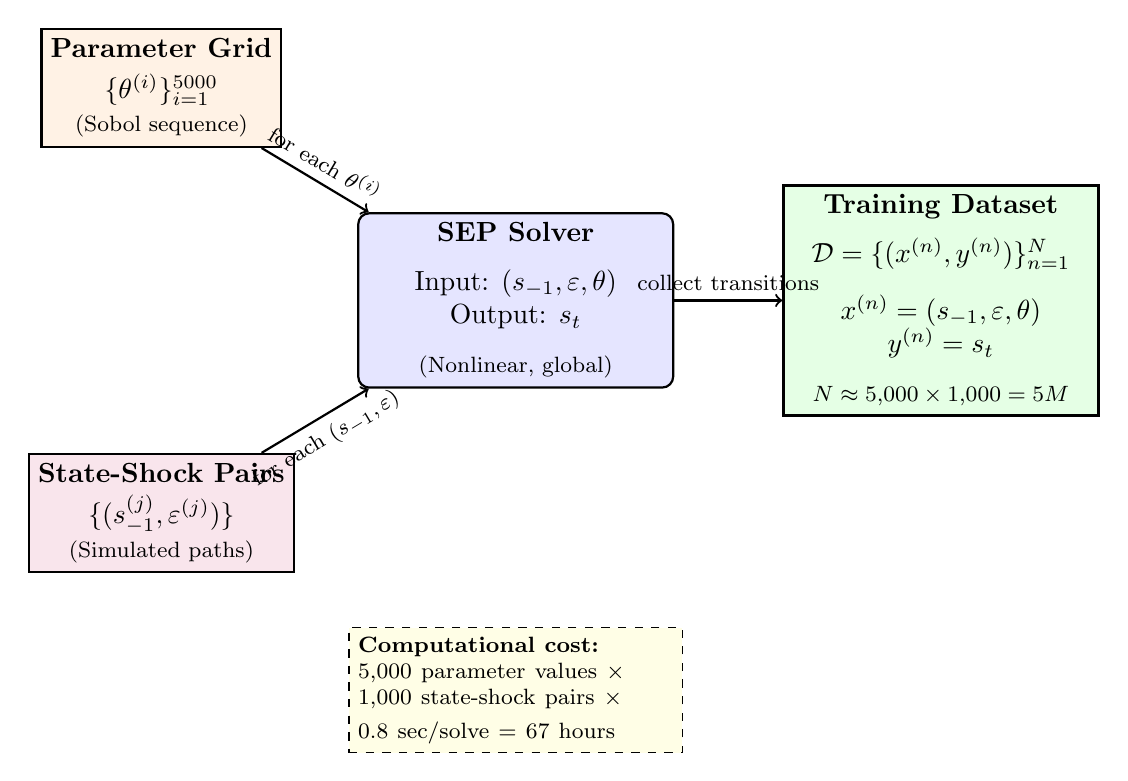
\begin{tikzpicture}[scale=0.9]

% SEP Solver Box
\node[draw, thick, rounded corners, fill=blue!10, minimum width=4cm, minimum height=2cm, align=center] (sep) at (0,0) {
  \textbf{SEP Solver} \\[2mm]
  Input: $(s_{-1}, \varepsilon, \theta)$ \\
  Output: $s_t$ \\[2mm]
  \footnotesize (Nonlinear, global)
};

% Parameter Grid
\node[draw, thick, fill=orange!10, minimum width=3cm, minimum height=1.5cm, align=center] (grid) at (-5,3) {
  \textbf{Parameter Grid} \\[1mm]
  $\{\theta^{(i)}\}_{i=1}^{5000}$ \\
  \footnotesize (Sobol sequence)
};

% State-Shock Samples
\node[draw, thick, fill=purple!10, minimum width=3cm, minimum height=1.5cm, align=center] (samples) at (-5,-3) {
  \textbf{State-Shock Pairs} \\[1mm]
  $\{(s_{-1}^{(j)}, \varepsilon^{(j)})\}$ \\
  \footnotesize (Simulated paths)
};

% Training Dataset
\node[draw, thick, fill=green!10, minimum width=4cm, minimum height=2.5cm, align=center] (dataset) at (6,0) {
  \textbf{Training Dataset} \\[2mm]
  $\mathcal{D} = \{(x^{(n)}, y^{(n)})\}_{n=1}^N$ \\[3mm]
  $x^{(n)} = (s_{-1}, \varepsilon, \theta)$ \\
  $y^{(n)} = s_t$ \\[2mm]
  \footnotesize $N \approx 5{,}000 \times 1{,}000 = 5M$
};

% Arrows
\draw[->, thick] (grid) -- (sep) node[midway, above, sloped] {\footnotesize for each $\theta^{(i)}$};
\draw[->, thick] (samples) -- (sep) node[midway, below, sloped] {\footnotesize for each $(s_{-1}, \varepsilon)$};
\draw[->, thick] (sep) -- (dataset) node[midway, above] {\footnotesize collect transitions};

% Annotation
\node[draw, dashed, fill=yellow!10, text width=4cm, align=left] at (0,-5.5) {
  \footnotesize \textbf{Computational cost:} \\
  $5{,}000$ parameter values $\times$ \\
  $1{,}000$ state-shock pairs $\times$ \\
  $0.8$ sec/solve = 67 hours
};

\end{tikzpicture}
\caption{From SEP Solutions to Training Dataset}
\label{fig:sep_to_training}
\begin{flushleft}
\footnotesize
\textbf{Notes}: Illustration of the dataset generation pipeline. For each parameter value $\theta^{(i)}$ in a Sobol-sequence grid, we simulate the model at $1{,}000$ randomly sampled state-shock pairs $(s_{-1}, \varepsilon)$. Each SEP solution produces a training pair $(x, y) = ((s_{-1}, \varepsilon, \theta), s_t)$. The complete dataset contains $\approx 5$ million input-output pairs, capturing the parameter-conditional transition map $g_\theta(s_{-1}, \varepsilon)$ across the prior support.
\end{flushleft}
\end{figure}

\clearpage

% Figure 3: MLP Architecture
\begin{figure}[h]
\centering
\begin{tikzpicture}[
  scale=0.9,
  layer/.style={draw, thick, rounded corners, minimum height=8mm, align=center},
  neuron/.style={circle, draw, minimum size=5mm, fill=blue!20},
  arrow/.style={->, thick}
]

% Input Layer
\node[layer, fill=orange!20, minimum width=3cm] (input) at (0,0) {
  \textbf{Input Layer} \\
  $\mathbb{R}^{29}$
};

\node[below=1mm of input, text width=3.5cm, align=center, font=\footnotesize] {
  $s_{-1}$ (22 dim) + \\
  $\varepsilon$ (4 dim) + \\
  $\theta$ (3 dim)
};

% Hidden Layer 1
\node[layer, fill=purple!20, minimum width=3cm] (hidden1) at (5,0) {
  \textbf{Hidden Layer 1} \\
  $\mathbb{R}^{256}$
};

\node[below=1mm of hidden1, font=\footnotesize] {tanh activation};

% Hidden Layer 2
\node[layer, fill=purple!20, minimum width=3cm] (hidden2) at (10,0) {
  \textbf{Hidden Layer 2} \\
  $\mathbb{R}^{128}$
};

\node[below=1mm of hidden2, font=\footnotesize] {tanh activation};

% Output Layer
\node[layer, fill=green!20, minimum width=3cm] (output) at (15,0) {
  \textbf{Output Layer} \\
  $\mathbb{R}^{22}$
};

\node[below=1mm of output, font=\footnotesize] {$s_t$ (next state)};

% Connections
\draw[arrow] (input) -- (hidden1) node[midway, above, font=\footnotesize] {$W_1 \in \mathbb{R}^{256 \times 29}$};
\draw[arrow] (hidden1) -- (hidden2) node[midway, above, font=\footnotesize] {$W_2 \in \mathbb{R}^{128 \times 256}$};
\draw[arrow] (hidden2) -- (output) node[midway, above, font=\footnotesize] {$W_3 \in \mathbb{R}^{22 \times 128}$};

% Parameter count
\node[draw, dashed, fill=yellow!10, text width=5cm, align=left] at (7.5,-3) {
  \footnotesize \textbf{Total parameters:} \\[1mm]
  $(29 \times 256) + 256 =$ 7,680 \\
  $(256 \times 128) + 128 =$ 32,896 \\
  $(128 \times 22) + 22 =$ 2,838 \\[1mm]
  \textbf{Total: 43,414 parameters}
};

% Forward pass
\node[draw, fill=blue!5, text width=6cm, align=left] at (7.5,-5.5) {
  \footnotesize \textbf{Forward pass:} \\[1mm]
  $h_1 = \tanh(W_1 x + b_1)$ \\
  $h_2 = \tanh(W_2 h_1 + b_2)$ \\
  $\hat{s}_t = W_3 h_2 + b_3$
};

\end{tikzpicture}
\caption{Neural Network Surrogate Architecture}
\label{fig:mlp_architecture}
\begin{flushleft}
\footnotesize
\textbf{Notes}: Schematic of the feedforward multilayer perceptron (MLP) used to approximate the SEP transition map. The network takes as input the previous state $s_{-1}$ (22 variables), current shock $\varepsilon$ (4 variables), and structural parameters $\theta$ (3 estimated parameters), for a total input dimension of 29. Two hidden layers with 256 and 128 neurons (tanh activation) provide nonlinear feature extraction. The output layer produces the next state $s_t$ (22 variables). All inputs and outputs are standardized to zero mean and unit variance during training.
\end{flushleft}
\end{figure}

\clearpage
